\documentclass[aps,pre,superscriptaddress]{revtex4}

\usepackage{preamble}
\graphicspath{ {./figures} }

\begin{document}

% \begin{abstract}
% \end{abstract}

\title{SBM-WCC Ian's Document}
\author{Ian Chen}
\date{\today}
\maketitle

\section{Introduction}
See the preprint~\cite{Park25-02}.

\section{Materials and Methods}

\section{Statistics}

\begin{figure}[ht]
	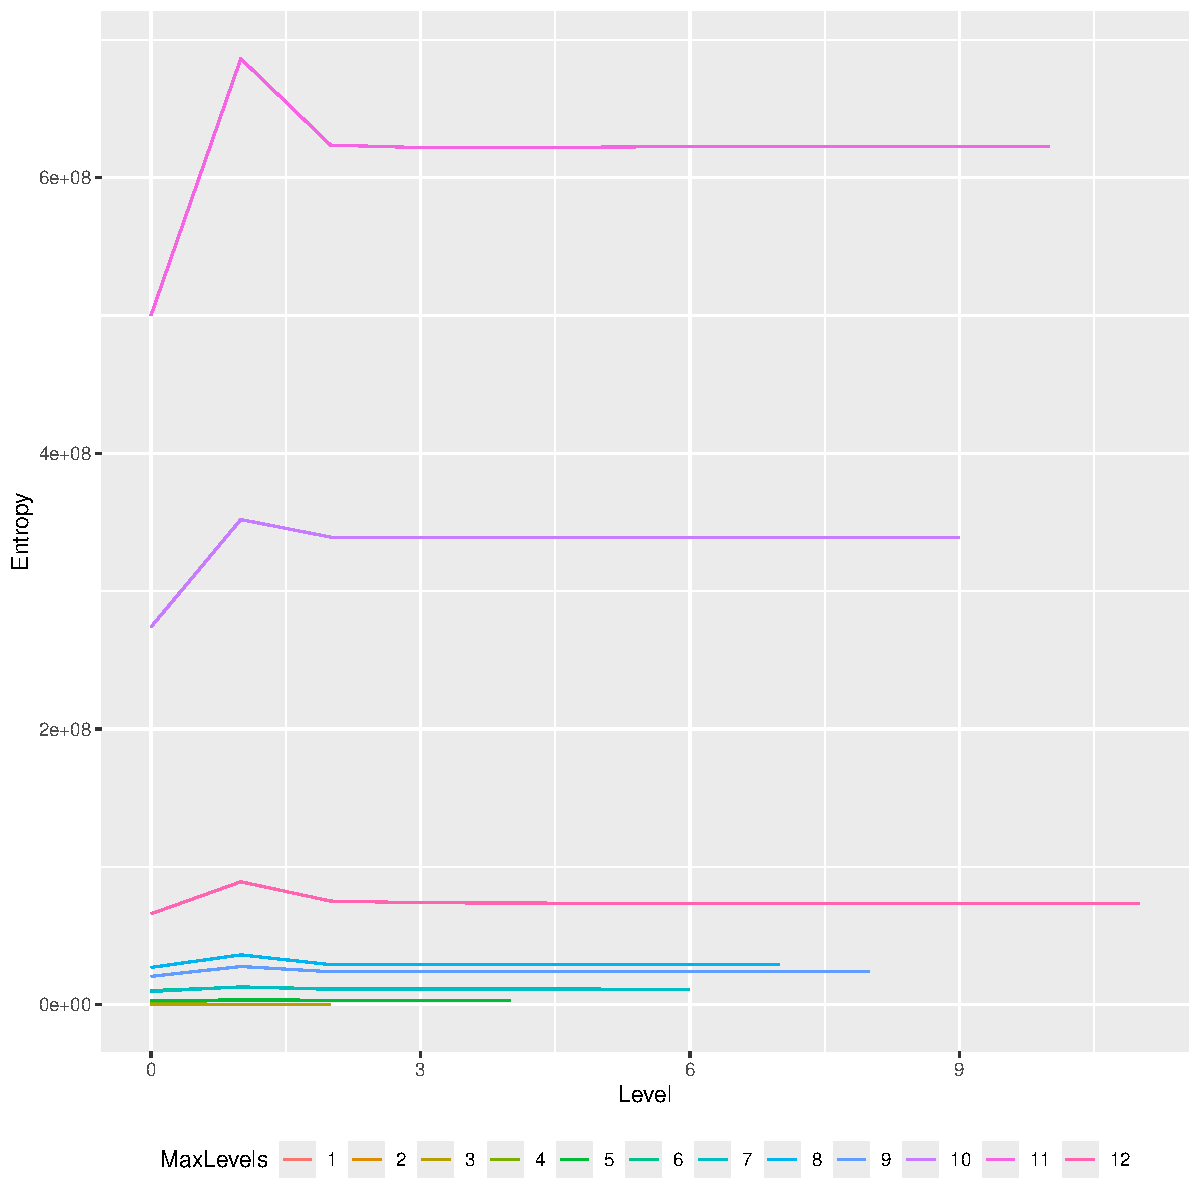
\includegraphics[width=\textwidth]{fig1.pdf}
	\caption{Connectivity of Hierarchical-SBM Clusters. Top: Level0. Bot: Level1.
		Each bar is a network, sorted in increasing network size.
		The y-axis shows percentage disconnected, poorly-connected $\setminus$ disconnected, and well-connected}
	\label{figs:fig1}
\end{figure}

\begin{figure}[ht]
	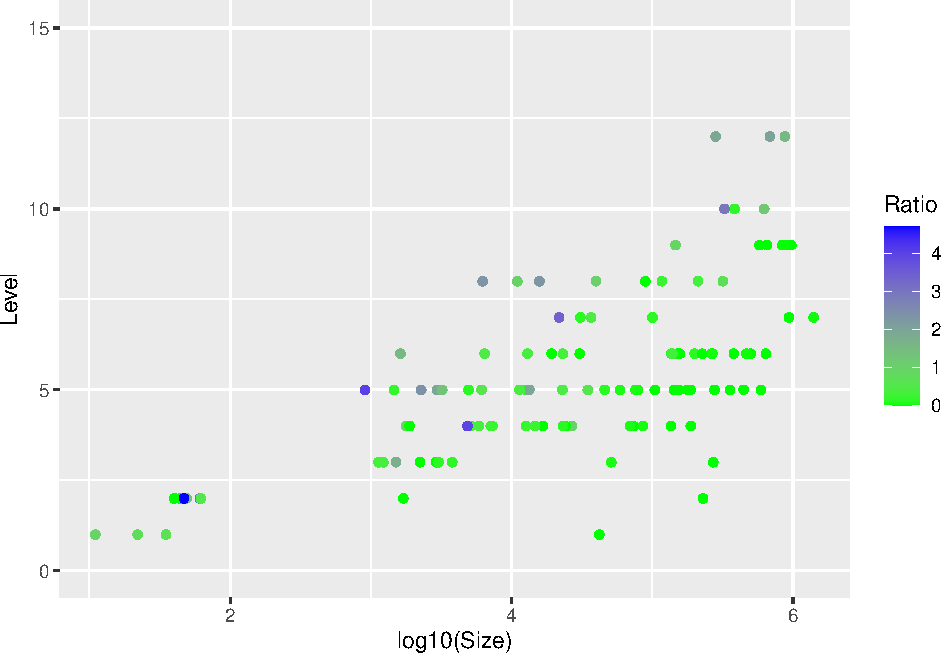
\includegraphics[width=\textwidth]{fig2.pdf}
	\caption{Levels of Hierarchical-SBM.
		Each point is a network.
		The x-axis shows the size of the network.
		The y-axis is the number of levels inferred in Hierarchical-SBM.
		We calculate the ClusterSize / $\log_{10}$ NetworkSize, so that a ratio of $>1$ is well-connected, and report the mean across the clusters in level 0 as the color.}
	\label{figs:fig2}
\end{figure}

\begin{figure}[ht]
	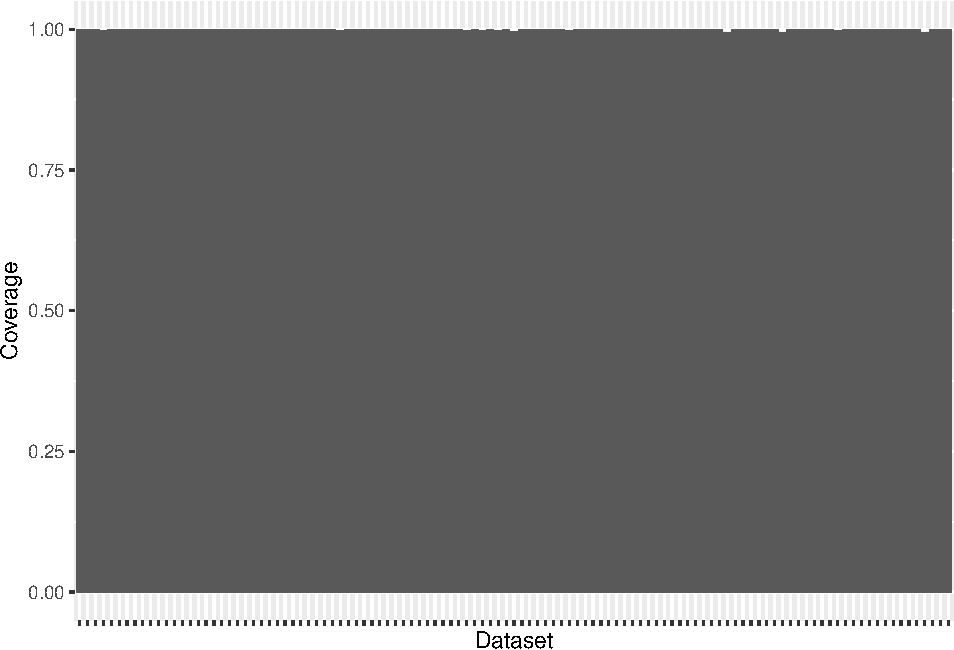
\includegraphics[width=\textwidth]{fig3.pdf}
	\caption{Node Coverage of Level0:
		Each bar is a network, sorted in increasing network size.
		The y-axis shows the node coverage, i.e. the percentage of nodes not in singleton clusters.}
	\label{figs:fig3}
\end{figure}

\begin{figure}[ht]
	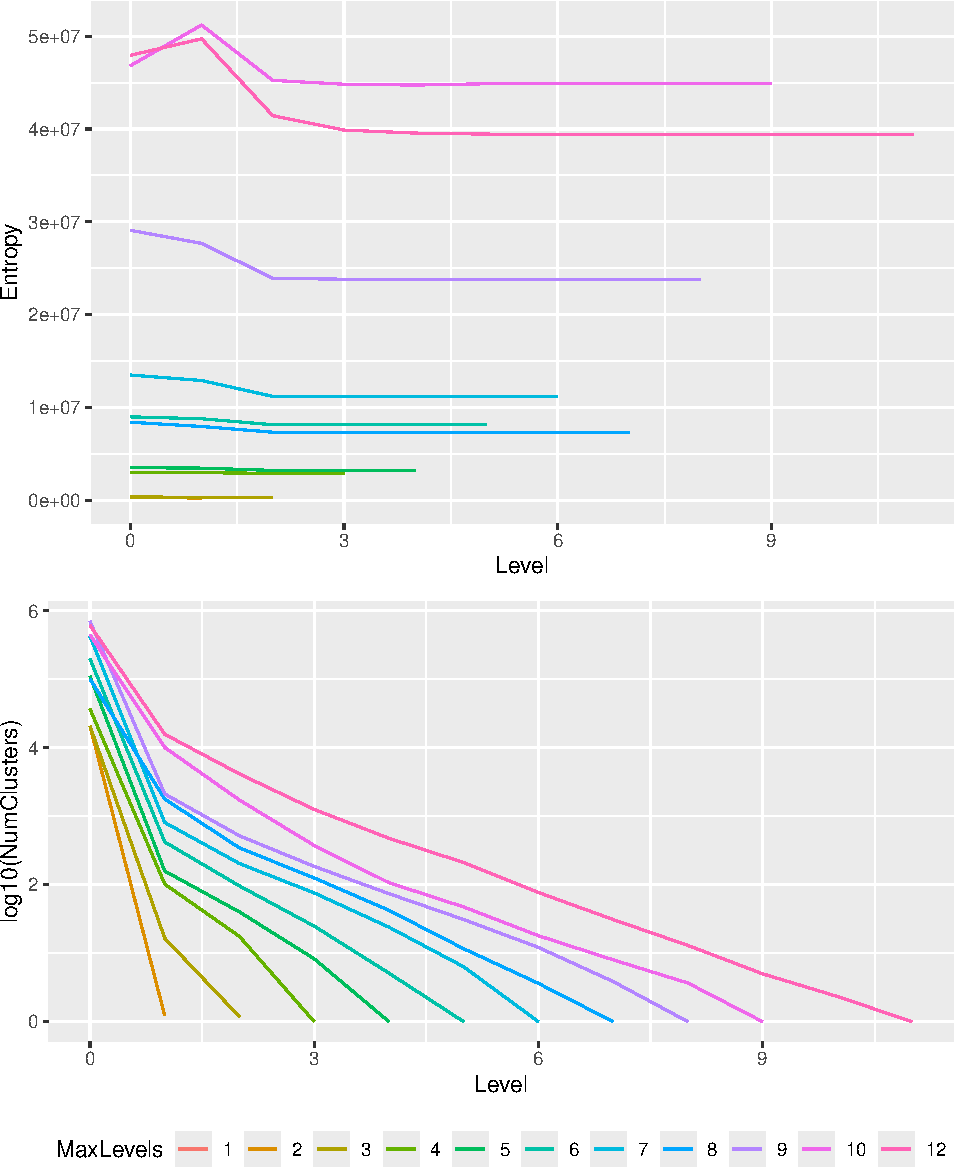
\includegraphics[width=\textwidth]{fig4.pdf}
	\caption{Description Length and Clusters across Levels:
		For each plot, we take the mean across all networks with MaxLevels number of inferred levels.
		Top: The description length is calculated according to the Degree Corrected (non-nested) SBM model.
		Bot: The number of clusters (log scale).}
	\label{figs:fig4}
\end{figure}

Examining just the cluster statistics for Hierarchical-SBM level0, we see that most networks exhibit mostly disconnected clusters (Figure \ref{figs:fig1}).
This problem is much worse when we go to level1.
TODO: compare to the DC-SBM.

Hierarchical-SBM has a trend of inferring more layers as the network size gets larger (Figure \ref{figs:fig2}).
Moreover, we see that the networks with clusterings that are mostly connected are generally those with disproportionately high number of levels for their size.
Hierarchical-SBM also generates clusterings with very high node coverage --- nearly 100\% across all networks (Figure \ref{figs:fig3}).

Examining the properties across levels, we see that the larger levels have much fewer clusters, and presumably larger clusters (Figure \ref{figs:fig4}).
I'm not sure what to make of the description length plateau as we increase levels?
Note that a lower description length is favored by the model.
TODO: compare the values with the DC-SBM values.
TODO: plot the cluster sizes too.

\section{Comparison}

Now, we compare Nested-SBM with DC-SBM without nesting.

\clearpage
\bibliography{refs}
\bibliographystyle{ACM-Reference-Format}

\end{document}
